The \textit{Repository Management} module is responsible for management and cataloging of
algorithms and test data to be used in the benchmarking tests.

\subsection{Domain Model}
The domain model for the Repository Management module is shown in Figure \ref{fig:repoManDomain}
\begin{figure}[H]
  \begin{center}
  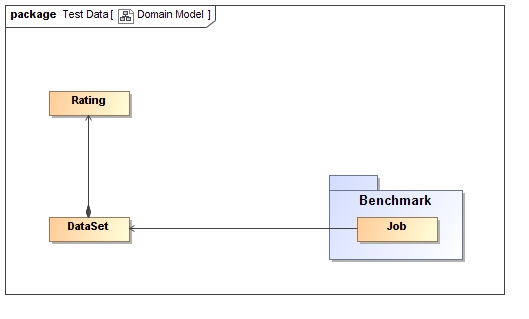
\includegraphics[scale=0.5]{../Diagrams and Charts/Test Data/Domain Model.jpg}  
  \caption{Repository Management Domain Model}
  \end{center}
  \label{fig:repoManDomain}
\end{figure}
\clearpage
\subsection{Scope}
The scope for the Repository Management module is shown in Figure \ref{fig:repoManScope}
\begin{figure}[H]
  \begin{center}
  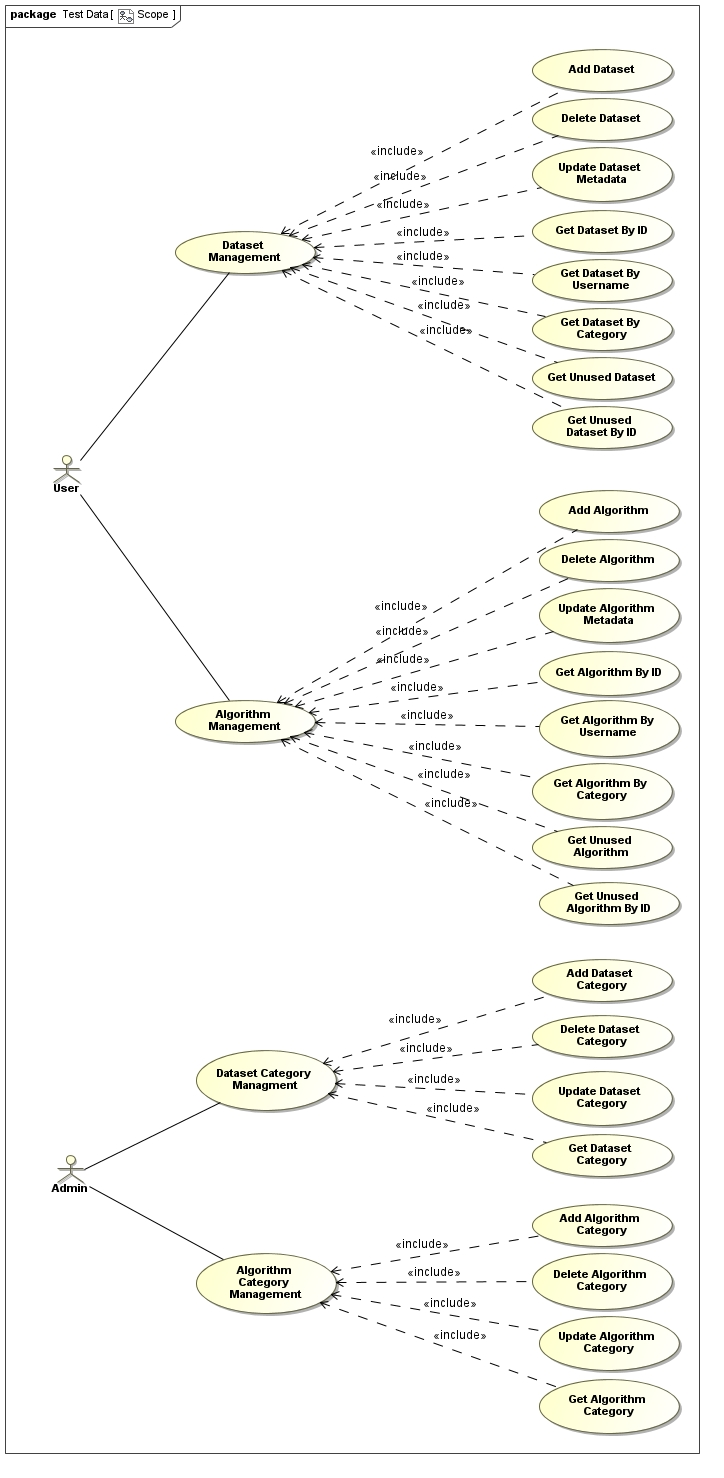
\includegraphics[scale=0.34]{../Diagrams and Charts/Test Data/Scope.jpg}
  \caption{Scope of Categories}
  \end{center}
  \label{fig:repoManScope}
\end{figure}

\subsection{Dataset Management}

\subsubsection {Users will be able to add a dataset}
The service contract for adding a dataset is shown in Figure \ref{fig:addDatasetService}
\begin{figure}[H]
  \begin{center}
  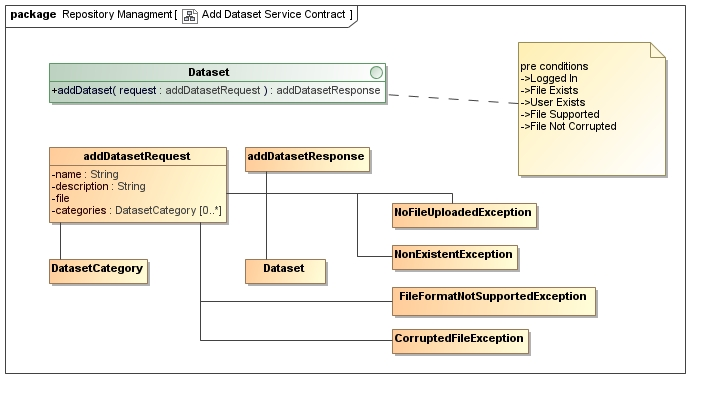
\includegraphics[scale=0.6]{../Diagrams and Charts/Test Data/Add Dataset Service Contract.jpg}
  \caption{Add Dataset Service Contract}
  \end{center}
  \label{fig:addDatasetService}
\end{figure}

\subsubsection {Users will be able to delete a dataset}
\subsubsection {Users will be able to update a dataset}
\subsubsection {Users will be able to get a dataset by ID}
\subsubsection {Users will be able to get a dataset by name}
\subsubsection {Users will be able to get a dataset by category}
\subsubsection {Users will be able to get all unused datasets}
\subsubsection {Users will be able to get an unused dataset by ID}

\subsection{Algorithm Management}

\subsubsection {Users will be able to add an algorithm}
\subsubsection {Users will be able to delete an algorithm}
\subsubsection {Users will be able to update an algorithm}
\subsubsection {Users will be able to get an algorithm by ID}
\subsubsection {Users will be able to get an algorithm by name}
\subsubsection {Users will be able to get an algorithm by category}
\subsubsection {Users will be able to get all unused algorithms}
\subsubsection {Users will be able to get an unused algorithm by ID}

\subsection{Dataset Category Management}

\subsubsection {Admin will be able to add a dataset category}
\subsubsection {Admin will be able to delete a dataset category}
\subsubsection {Admin will be able to update a dataset category}
\subsubsection {Admin will be able to get a dataset category}

\subsection{Algorithm Category Management}

\subsubsection {Admin will be able to add a algorithm category}
\subsubsection {Admin will be able to delete a algorithm category}
\subsubsection {Admin will be able to update a algorithm category}
\subsubsection {Admin will be able to get a algorithm category}







